\documentclass[10pt]{article}
\usepackage[a4paper,margin=17mm]{geometry}
\usepackage{amsmath,amssymb,booktabs,graphicx,microtype,xcolor}
\usepackage[colorlinks=true,urlcolor=blue,citecolor=blue,linkcolor=blue]{hyperref}
\setlength{\parindent}{0pt}\setlength{\parskip}{3.5pt}
\newcommand{\meV}{\,\mathrm{meV}}
\newcommand{\dd}{\mathrm d}
\title{Finite collection and readout loss in a radiative wire-plasma haloscope}
\author{Independent numerical assessment}
\date{18 October 2026}
\begin{document}
\begin{center}
{\Large Finite collection and readout loss in a radiative wire-plasma haloscope}\\[6pt]
Independent numerical assessment --- 18 October 2026
\end{center}
\textbf{Finding.} A radiative wire stack has a concrete opportunity at meV masses when it avoids a sparse pickup system or a sufficiently lossy guided output. A dense, lossless distributed receiver removes the sparse-pickup advantage. At equal active volume, the strongest tested port benchmark has about twice the intrinsic scan response of the radiative design. With an additional optical power transmission of 0.8, only 2.3--2.9\,dB of port-chain loss is required to reverse that ordering. The calculated transport threshold becomes much shorter at higher mass. This supports a prototype aimed at measuring extraction and transmission. It does not establish superiority over every possible implementation of ALPHA.

\section{What is compared}
The physical issue is transport inside a lossy plasma. Let $Q_u=\omega U/P_{\rm ohm}$ be the unloaded quality factor, with stored energy $U$ and ohmic power loss $P_{\rm ohm}$. Near the plasma frequency, the bulk amplitude attenuation length is approximately $\lambda\sqrt{2Q_u}/(2\pi)$~\cite{alpha}. For the adopted copper model it is about 6.3, 2.5 and 1.0\,mm at 1, 2 and $4\meV$. A localized receiver does not automatically collect power from the entire axion-driven volume. Distributed pickups can do so; a radiating face offers another route by letting each part of the aperture couple to external optics. The attenuation length is neither a maximum apparatus size nor a prescribed pickup spacing.

Both devices use a $10\,\mathrm{cm}\times10\,\mathrm{cm}$ face, the same static field and axion density, and copper with the common assumed surface resistance
\begin{equation}
 R_s(\nu)=1.8(2.9\,\mathrm{m}\Omega)
 \left(\frac{\nu}{3.9\,\mathrm{GHz}}\right)^{2/3},\qquad
 \nu_a=241.799\,\mathrm{GHz}\,\frac{m_a}{1\meV}.
 \label{eq:rs}
\end{equation}
Equation~\eqref{eq:rs} retains the manuscript's engineering allowance for surface and field losses; it is an assumption to test, not a new THz measurement. The radius-to-pitch ratio is 0.03 in both starting designs. The four masses below are comparison points, not physical mass limits. The established sensitivity forecast extends below $0.5\meV$ and is unchanged by this assessment.

The radiative calculation resolves vector fields in a finite sheet enclosure, with a conducting back and side walls, an open face in an infinite conducting flange, and collection into one external Gaussian mode. It includes propagation between sheets and diffraction within this macroscopic model. Circular wire surfaces, contacts, supports and finite-flange optics are not resolved. For each mass, the grid count is selected from $N=5,\ldots,24$ by maximizing the one-dimensional frequency-integrated squared power response at fixed face area; the selected design is then evaluated with the finite-aperture solver. The Gaussian waist is optimized. Thus the grid counts follow a stated objective and are not imposed.

\begin{center}
\begin{tabular}{rrrrrr}
\toprule
$m_a$ [meV] & $N$ & Pitch [$\mu$m] & Diameter [$\mu$m] & Depth $L$ [mm] & $\eta_{\mathcal I}$\\
\midrule
0.5 & 14 & 669.3 & 40.16 & 9.370 & 0.722\\
1 & 12 & 335.5 & 20.13 & 4.026 & 0.761\\
2 & 10 & 168.5 & 10.11 & 1.685 & 0.777\\
4 & 9 & 84.49 & 5.069 & 0.761 & 0.779\\
\bottomrule
\end{tabular}
\end{center}
Here $\eta_{\mathcal I}=\sqrt{\mathcal I_G/\mathcal I_{\rm 1D}}$ compares collection into the Gaussian mode with the one-dimensional response. These numbers are calculated collection factors, not the fixed 0.65 forecast input. They are consistent with retaining that input at the checked settings.

The port comparator is a finite rectangular Drude plasma, with perfectly conducting boundaries, wires parallel to the electric field, and explicit spatial pickup profiles. It follows the plasma description used in the ALPHA design study~\cite{alpha}, but it is an independently constructed benchmark, not an ALPHA hardware design. We allow $K=1,4,16,64$ Gaussian pickup columns and a continuous-profile receiver. Each column extends along the wires. Their outputs feed \emph{one ideal coherent receiver}; no detector-noise penalty is assigned for increasing $K$. The reactive load and extraction strength are searched, and the plasma frequency is retuned so the loaded resonance is at the comparison mass. The pickup width is initially twice the wire pitch. Varying it from one to four pitches is a separate sensitivity check.

For equal active volume, the comparator occupies the same depth $L$ as the stack. A second comparison lets it fill 30\,mm of depth while retaining one radiating face for the grid design. This exposes the cost of leaving magnet volume unused. It is a rectangular-box benchmark, not a simulation of a conformal solenoidal optical system.

\section{The quantity that controls sensitivity}
Let $b(\nu)$ be the output signal power divided by the power from a bare mirror of the same face area. The latter is normalized to a numerical coupling,
\begin{equation}
 \frac{P_{\rm mir}}{A}=7.33\times10^{-26}\,\frac{\mathrm W}{\mathrm m^2}
 \left(\frac{g_{a\gamma}}{10^{-12}\,\mathrm{GeV}^{-1}}\right)^2
 \left(\frac{B_0}{10\,\mathrm T}\right)^2
 \frac{\rho_a}{0.4\,\mathrm{GeV\,cm}^{-3}}
 \left(\frac{1\meV}{m_a}\right)^2.
\end{equation}
Define $\mathcal I=\int b(\nu)^2\dd\ln\nu$. For slowly varying white output noise and locally translated tuning spectra, the scan rate is proportional to this integral. If $\eta_r$ and $\eta_p$ are the additional power transmissions after the radiative and port outputs, and $S_r,S_p$ their output noise spectral densities, the local scan-rate ratio is
\begin{equation}
 R\simeq R_0\left(\frac{\eta_r}{\eta_p}\right)^2
              \left(\frac{S_p}{S_r}\right)^2,
 \qquad R_0=\frac{\mathcal I_r}{\mathcal I_p}.
 \label{eq:ratio}
\end{equation}
At fixed live time, $g_{\min,r}/g_{\min,p}=R^{-1/4}$. We integrate the spectra over $0.85<\nu/\nu_a<1.15$. A second integral restricted between the half-maximum crossings checks a one-FWHM counting filter, where FWHM denotes full width at half maximum. Its dense-port ratios differ from the full-band ratios by about 1--2\%. These are local response comparisons, not new complete octave-by-octave forecasts.

The table includes the same Gaussian halo used in the forecast: one-dimensional velocity dispersion $220/\sqrt2\,\mathrm{km\,s}^{-1}$ and a transverse wind of $232\,\mathrm{km\,s}^{-1}$. Each device's reciprocal receiving field determines its overlap. The peak overlap multiplies the narrow-resonance scan integral; the port overlap changes by less than 0.5\% across the FWHM. Phase across the thin radiative depth is neglected. All quoted ratios below use equal additional transmission and equal output noise.

\begin{center}
\begin{tabular}{rrrrrr}
\toprule
& \multicolumn{5}{c}{$R_0$, same active volume}\\
$m_a$ [meV] & $K=1$ & $K=4$ & $K=16$ & $K=64$ & Continuous\\
\midrule
0.5 & 4.17 & 0.547 & 0.457 & 0.415 & 0.426\\
1 & 31.5 & 1.94 & 0.495 & 0.465 & 0.462\\
2 & 198 & 14.2 & 0.889 & 0.534 & 0.525\\
4 & 839 & 87.5 & 5.59 & 0.562 & 0.543\\
\bottomrule
\end{tabular}
\end{center}
Values above unity favor radiative collection. The very large single-pickup ratios quantify the failure of that particular sparse receiver to collect a broad source. They are not advantages over an optimized distributed plasma haloscope. The continuous profile is a favorable idealization for the comparator, and the finite-$K$ results describe the specified profile family rather than a minimum required antenna count. The ALPHA study itself permits multiple antennas~\cite{alpha}; its current Phase I design targets 10--20\,GHz~\cite{phase1}. Neither observation fixes the achievable meV readout.

\begin{figure}[ht]
\centering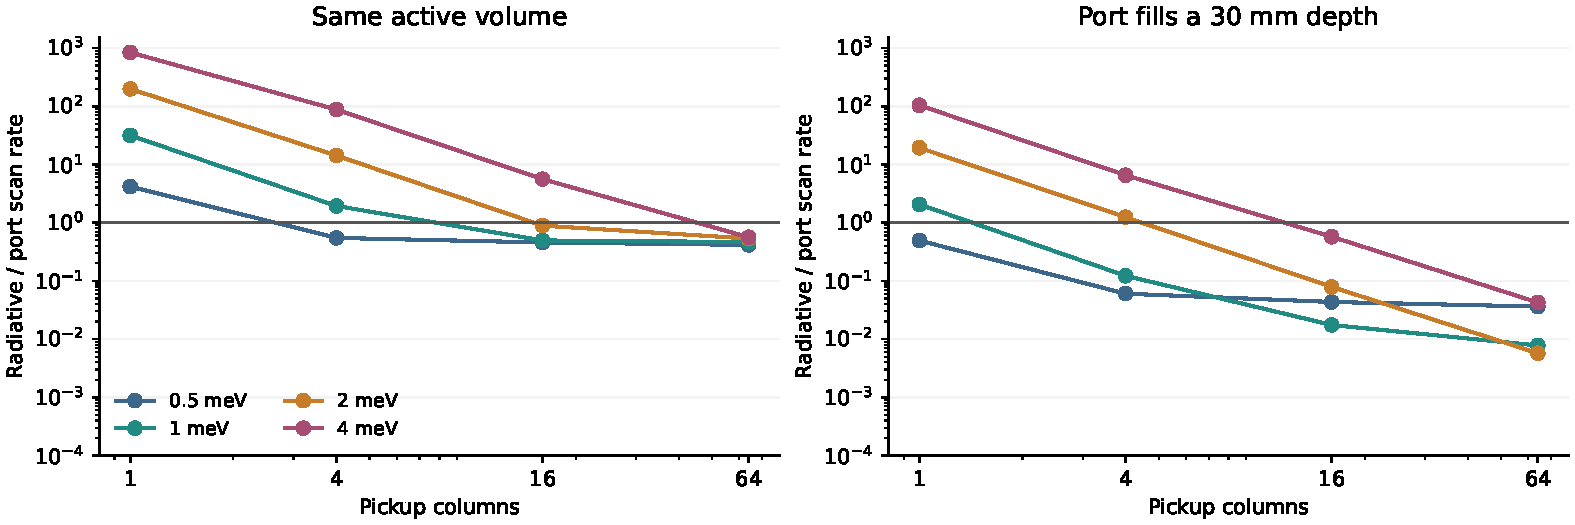
\includegraphics[width=\linewidth]{figures/pickup_comparison.pdf}
\caption{The same source-driven port calculation in two resource comparisons. Each curve allows an ideal one-output coherent network. The right panel gives the port design extra active depth; the radiative design still has one emitting face. The pickup count is therefore a displayed engineering variable, not a hard restriction used to claim a universal advantage.}
\end{figure}

\section{A quantitative target for a prototype}
Against the strongest tested port profile, set $\eta_r=0.8$ as an explicit optical target and take equal output noise. The port power loss at parity is $\mathcal L_p=-10\log_{10}(0.8\sqrt{R_0})$ in decibels. This criterion can be measured directly, without assuming that ALPHA must use a particular pickup spacing.

\begin{center}
\begin{tabular}{rrrrr}
\toprule
& \multicolumn{2}{c}{Same active volume} & \multicolumn{2}{c}{Port fills 30\,mm}\\
$m_a$ [meV] & Loss [dB] & Guide length [cm] & Loss [dB] & Guide length [cm]\\
\midrule
0.5 & 2.88 & 153 & 8.22 & 438\\
1 & 2.65 & 44.4 & 11.90 & 200\\
2 & 2.37 & 12.5 & 15.49 & 81.9\\
4 & 2.30 & 3.83 & 18.81 & 31.3\\
\bottomrule
\end{tabular}
\end{center}
The lengths are an illustration, calculated for a common output guide \emph{after} an ideal combiner. They assume a rectangular copper guide of width $a_w$, height $b_w=a_w/2$, and operating frequency $\nu/\nu_c=1.7$, where $\nu_c=c/(2a_w)$ is the fundamental-mode cutoff. With vacuum impedance $Z_0$, the amplitude attenuation is~\cite{guide}
\begin{equation}
 \alpha_c=\frac{R_s}{Z_0 b_w}
 \frac{1+(2b_w/a_w)(\nu_c/\nu)^2}{\sqrt{1-(\nu_c/\nu)^2}},
 \qquad \eta_p=\exp(-2\alpha_c\ell).
 \label{eq:guide}
\end{equation}
Here $\ell$ is guide length. The assumed $R_s\propto\nu^{2/3}$ and transverse dimensions proportional to $\nu^{-1}$ give $\alpha_c\propto\nu^{5/3}$. The calculated power losses are 1.88, 5.96, 18.9 and 60.0\,dB/m at the four masses. Halving the guide surface resistance doubles each parity length. These losses are not assigned to ALPHA: overmoded guides, dielectric transport, superconducting sections or a quasi-optical output can change them.

For example, at $2\meV$, a 20\,cm guide with the stated copper loss and an 80\% optical path give $R\simeq1.92$ at equal active volume, or an approximately 15\% improvement in coupling reach at fixed time. At $4\meV$, the parity length is only about 4\,cm. These are explicit conditional advantages. If a port design can exploit the full 30\,mm depth, the volume gain is much harder to overcome; the last two columns quantify that condition. A claimed fixed-magnet advantage must demonstrate that gain survives the actual optical layout and usable volume.

A useful first electromagnetic prototype is the $1\meV$ geometry in the first table: twelve grids, approximately $336\,\mu$m pitch and $20\,\mu$m wire diameter. Measure the resonance frequency, response width, Gaussian collection and the competing guided path. An absorption measurement alone does not determine axion overlap: use reciprocal field mapping and a calibrated electromagnetic model to determine the volume overlap with the static field. Cryogenic quasi-optical S-parameter measurements in the 220--330\,GHz band already provide a relevant measurement methodology~\cite{quasioptic}. The material loss must ultimately be checked in the intended magnetic field, and all photon-counting paths must satisfy the background budget.

\section{Verification and scope}
The port solution conserves source work to better than $10^{-13}$ in the tested cases. An independent two-dimensional finite-difference solution agrees to 0.049\% in received power; refining the modal basis from 2272 to 8773 modes changes the checked scan integral by less than $10^{-5}$ relative. The isolated-mode limit recovers the scan-optimal external-to-internal damping ratio of two. For radiation at $1\meV$, refining 60 to 80 modes and the aperture quadrature changes the checked central integral by 0.0036\%. At $4\meV$, a paraxial-admittance check raises that integral by about 2\% from 60 to 240 modes. The highest-mass ratios therefore have few-percent numerical precision, separately from hardware-model uncertainty.

The port uses a passive homogenized network; the radiator uses macroscopic sheets. Resolved probes, contacts, supports and manufactured optics remain to be studied. Geometry, material losses, mode engineering and magnet layout can improve either device. The practical criterion is that \emph{radiative extraction deliver a broad aperture to one low-noise receiver with less loss or less collection hardware than a competing distributed readout.} Code, raw spectra and checks accompany this note. The absolute coupling forecast is unchanged.

\begin{thebibliography}{9}\small
\bibitem{alpha} A. J. Millar et al., \emph{Searching For Dark Matter with Plasma Haloscopes}, \href{https://arxiv.org/abs/2210.00017}{arXiv:2210.00017}.
\bibitem{phase1} ALPHA Collaboration, \emph{Design of ALPHA Phase I: A Plasma Haloscope for 10--20 GHz Post-Inflation Axions}, \href{https://arxiv.org/abs/2608.10292}{arXiv:2608.10292}.
\bibitem{guide} N. Marcuvitz, \emph{Waveguide Handbook}, ch. 2; conductor-loss formula also given in the \href{https://scikit-rf-official.readthedocs.io/en/v2.1.0/api/media/generated/skrf.media.rectangularWaveguide.RectangularWaveguide.alpha_c.html}{scikit-rf rectangular-waveguide documentation}.
\bibitem{quasioptic} M. Masyukov et al., \emph{Quasioptic, Calibrated, Full 2-port Measurements of Cryogenic Devices under Vacuum in the 220--330 GHz Band}, \href{https://arxiv.org/abs/2506.03824}{arXiv:2506.03824}.
\end{thebibliography}
\end{document}
